
\subsubsection{Molecular Marine Biology - Biodiagnostics for
Toxic Effects} \index{K�hler, Angela}

\paragraph{Research Team}
%
Angela K�hler (Adjunct Professor - International University Bremen /
MaCoPolI-AWI, Marine Biotechnologies-AWI):
Katja Broeg (Principal Scientist), Sivia Kodeih (Principal Scientist), Bela Buck (Postdoc), Markus Geisen (Postdoc), Christian Hamm (Postdoc), Christoph Baum (Postdoc), Sonja Einsporn (PhD Student), Sabine Sch�fer (PhD Student),  Nassos Athanassios (PhD Student), Ralf Fisch (PhD Student), Tanja Michler (PhD Student), Matthias Brenner  (PhD Student), G�nther Kr�ner (Engineer), Sieglinde Bahns (Lab Technician), Ute Marx (TEM Technician),  Steffi Meyer (Lab Technician) \\

\newpage
 Our research goals are to understand mechanisms of cell and tissue
injury by natural and man made chemicals in marine life. Seagoing
studies in various climate zones along contamination gradients
provide insights into the spectrum of responses in indicator species
towards the complex mixture of chemicals introduced into the marine
environment. Experimental exposure studies to hazardous chemicals
serve to identify specific biomarkers of interaction with chemicals
and of related toxic effects including carcinogenesis and
infertility. Biomedical tests and assays are developed for
application in marine organisms since years in our laboratories.
Patterns of cellular responses serve for the identification of
criteria for the assessment of environmental health in international
monitoring programmes such as OSPAR, HELCOM, MEDPOL and the UNEP.
The implementation of Marine Biotechnologies into the AWI structure
of New Technologies is the answer to increasing needs to exploit the
knowledge of biological processes and marine resources to be
channelled into technology transfer and new products from the sea.

\paragraph{Highlights}
%
The evolution of cellular defence mechanisms of marine organisms have once facilitated life in extreme biotopes such as hydrothermal environments characterised by high levels of metals and organic chemicals. Nowadays, the same strategies protect life against man made pollution. Those chemicals which destroy or inhibit these conserved protective mechanisms are qualified as especially hazardous by environmental agencies. \\
For example, marine organisms defend themselves against chemicals by transmembrane efflux pumps of a gene family of ABC transporters mediating multidrug resistance or multixenobiotic resistance (MXR). \\
Our results evidenced homologies of genes of the blue mussel to human genes in the nucleotide sequence of 69\% for Pgp, the most important human transporter also overexpressed in cancer cell as defence against chemotherapeutic drugs. During a field campaign mussels were captured at different Norwegian Fjord sites with high chemical point source input at a copper mining site and an aluminium smelter releasing high amounts of polycyclic hydrocarbons (PAHs). Whereas drug elimination was inhibited at the aluminium smelter site, the \textit{mrp} gene expression together with activity, involved in export of metal gluthathione conjugates was increased at the copper mining site indicating successful protection of the organisms against metal exposure. Based on the sequence information we now design specific antibodies directed against the various transporters to elucidate their localisation in various membranes including the lysosomal membrane.

\begin{figure}[ht]
  \begin{center}
   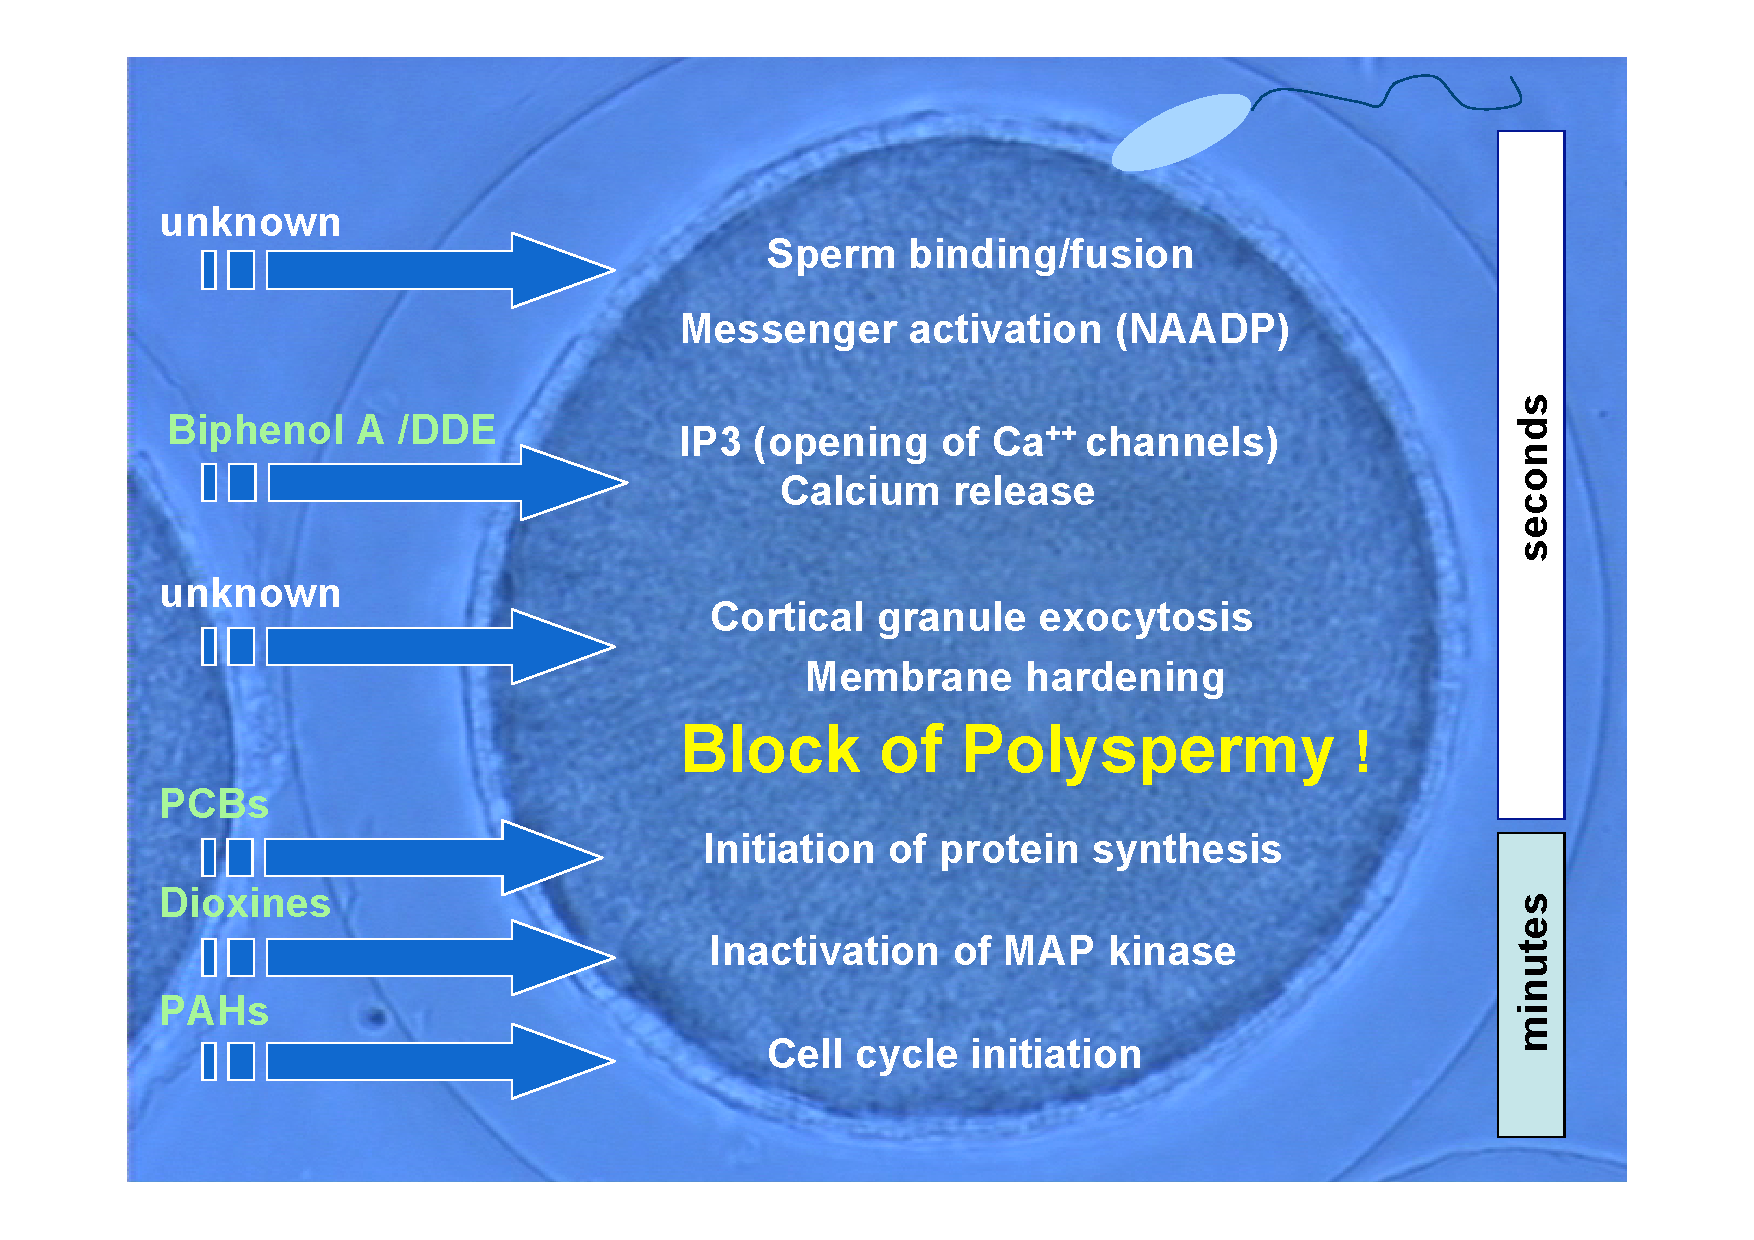
\includegraphics[width=\hsize]{Koehler/Koehler-2006FigA.png}
    \mycaption{Non-genomic interference of chemicals with successful fertilisation and embryonal development- (sea urchin eggs as models for human infertility). }\label{fig:Koehler-2006Fig}
   \end{center}
\end{figure}

The recently implemented section of Marine Biotechnologies in New Technologies under the AWI structure comprise topics related to Marine Structures and Nanomaterials, Natural Products and Biological Processes, Marine Aquaculture and Biodiagnostics. These topics have a joint source to be exploited in the observation of cellular structures, processes and their products. \\
The oceans host a multitude of organisms with highly complex structures. The well-founded knowledge of the biomechanic and structural properties of complex marine micro- and nanostructures e.g. shells and skeletons is now forming the basis for new lightweight structures and composites which are then readily available for applications in the automobile industry, airspace industry, shipbuilding, architecture and industry design for various applications.\\
With respect to offshore technology there is a worldwide shift of mariculture facilities from the protected coastal zone towards offshore regions- offshore- or open ocean aquaculture. For the realisation of such offshore constructions and -combinations techniques are developed at AWI which resist the harsh weather conditions (wave action and currencies, AWI patent) and are appropriate for the cultivation of marine organisms. The sites need a Monitoring-Program, with focus on especially security, protection of the ecosystem, management and improvement of the technique. \\
Marine biodiagnostics is based on the rapid advances in cell biology including the analysis of metabolic processes in marine organisms in response to specific life conditions. New concepts of marine environmental protection and monitoring of offshore industries and aquaculture as well as bioremediation of contaminated coastal areas and harbours  will be developed in collaboration with commercial enterprises. The development of new tools is focused on user friendly test kits for Tox- and BioSensors for the identification of chemical molecules in cells, organisms and food.


\paragraph{Organization}
%
\begin{enumerate}
\item {Head of Marine Biotechnologies to facilitate Technology Transfer out of AWI Biosciences}
\item {Head of AWI-research group Cell Biology and Toxicology in the MaCoPolI programm of the Helmholtz Society (HGF)}
\item {Member of the consortium to initiate a technology transfer platform and institute for the Bremen Senate}
\item {Member of the ICES Working Groups ``Biological Effects of Contaminants in Marine Organisms'' and ``Diseases in Marine  Organisms'' (OSPARCOM)}
\item {Member of the NADINE (Natural Disaster Network-Oil Accidents) platform of the Helmholtz Society (HGF)}
\item EU-workshop Bioinformatics I - Introduction to Sequence and Genome Analysis in collaboration with the Ribocon GmbH (January 23-27)
\item Extended international phylogeny (ARB) workshop in collaboration with the Ribocon GmbH (May 30 - June 02)
\item International Exploratory Workshop: ``Marine Genomics meets Marine Diversity'' (June 07-09)
\item International phylogeny (ARB) workshop in Z�rich in collaboration with the Ribocon GmbH (September 19-22)
\item International phylogeny (ARB) workshop in collaboration with the Ribocon GmbH (November 28 - December 02)
\end{enumerate}


\myparagraph{Collaborations}
Bremen Area Collaborations:
\begin{enumerate}
\item {\sl International University Bremen}\\Prof. K. Brix \\Hormonal effects of chemicals in sea urchins
 \\Prof. A. Koschinsky \\Cellular localisation of metals in hydrythermal organisms
\end{enumerate}
%
National \& International Collaborations:
\begin{enumerate}
\item {\sl Stanford University, Marine Station Pacific Grove, CA, USA} \\ Prof. D. Epel\\ Sea urchins as model of infertility in wildlife and humans
\item {\sl Rijksuniversiteit Groningen, The Netherlands}\\ Dr. H. Van der Want \\ Immunolocalisation by pre-embedding technique
\item {\sl University of Bilbao, Spain} \\ Prof. M. Cajaraville \\ Cancer diagnosis in fish after the Prestige oil spill, Natinal research project
\item {\sl Davis University, CA, USA} \\ Dr. I. Werner \\ Lysosomal membrane stability in insects
\item {\sl Stazione Zoologica ``A. Dohrn'', Italy} \\ Dr. A. Iannora \\ Defence mechanisms in copepod species against algae toxins
\item {\sl University of Allessandria and Genua, Italy} \\ Prof. A. Viarengo \\ Two tiered biomarker approach
\item {\sl Academic Medical Center, University of Amsterdam, The Netherlands} \\ Prof. C.J.F. Van Noorden \\ Postranslational regulation of enzymes of the PPP during fertilisation
\end{enumerate}


\paragraph{Grants at the Alfred Wegener Institute Bremerhaven}
\begin{enumerate}
\item EU Project Pallas Athene (2005-2007) Topic: Science goes public. Ambassador for Women in Science.

\item MYTIFIT (2005-2008) Eignung des Seegebietes am geplanten Offshore-Windpark ``Nordergr�nde'' f�r die Zucht von Miesmuscheln: Fitness, Parasitierung und Substratwahl. Angewandte Umweltforschung des Senats f�r Bau, Umwelt und Verkehr.

\item CANCERMAR (2006-2009) Mecanismos celulares y moleculares de carcinog�nesis qu�mica en organismos acu�ticos: aplicaciones para la evaluaci�n de la calidad del medio marino. Spanish Ministery of Education and Science.
\end{enumerate}

\paragraph{Patents}
\begin{enumerate}
\item{ Trademark Ovohard, Inner Market-registration No 004726758, 25/10 2006, Alicante Spain.
International registration - No 890732 4/08 2006, Geneva, Switzerland.}
\item{Subject:  Caviar processing without killing the female in the frame of conservation of endangered species (patent under review).}

\end{enumerate}

\nocite{Koehler1,Koehler2,Koehler3,Koehler4}
